In this chapter I will show the behaviour of task-affinity on different architectures. First of all, we will check if the expected scheduling is performed. 
After which we will analyze how the optimization proposed influences performance and L1 and LLC miss rates of the application. 

In Fig. \ref{fig:ideal_scheduling} the scheduling that vanilla and the developed patch should perform are represented.

\begin{figure}[htbp]
\centering
\includegraphics[width=\widefigure]{images/schedule_van_taskaff.eps}
\caption{\figurecaption{Ideal Scheduling performed by vanilla (left) and task-affinity (right).}}
\label{fig:ideal_scheduling}
\end{figure}

We have assumed that \textit{mixer0} and \textit{mixer1} have the same duration, all \textit{waves} have the same duration.
In the real benchmark, durations of the \textit{waves} are slightly different, durations of the \textit{mixer0} and 
\textit{mixer1} are slightly different. Furthermore we assume that \textit{mixer0} and \textit{mixer1} never start when \textit{waves} are still in 
execution.

Considering the time normalized to the duration of one sample, it is possible to express durations of different tasks in relative terms.
Using relative durations, it is possible to estimate the improvement given by task-affinity using \textit{amdhal's law} \cite{lcs}:

\begin{equation}
       Speedup = \left(\frac{P_{1}}{S_{1}} + \frac{P_{2}}{S_{2}} + ... \frac{P_{n}}{S_{n}} \right)^{-1} 
\label{eq:amdhal}
\end{equation}

Where $P_{i}$ is the $i-th$ parallelized portion of the program and $S_{i}$ is the correspondent parallelization factor. Furthermore the following 
constraint must be respected:

\begin{equation}
       \sum_{i=1}^N P_{i} = 1
\label{eq:contr_amdhal}
\end{equation}

Before to explain in which portions the serial execution of the benchmark is subdivided, it is necessary define some variables:

\begin{description}
\item[$T_{W}$:] average of execution time of a \textit{wave}
\item[$T_{M_{0,1}}$:] average of execution time of \textit{mixer0} and \textit{mixer1}
\item[$T_{M_{2}}$:] average of execution time of \textit{mixer2}
\item[$T_{W,M}$:] difference between $T_{M_{2}}$ and $T_{W}$ that is $T_{W,M} = T_{M_{2}} - T_{W}$
\end{description}

The serialized execution of benchmark can divided into the following portions:

\begin{table}[htbp]
\begin{center}
\begin{tabular}{|l|c|c|c|c|} \hline
& $P_{1}$ & $P_{2}$ & $P_{3}$ & $P_{4}$ \\ \hline
vanilla & $T_{M_{0,1}}*2$ & $T_{W}*4$ & $T_{M_{2}}$ & -- \\ \hline
\multirow{2}{*}{taskaff} & {$T_{M_{0,1}}*2$} & $3*T_{W} + T_{W,M}$ & $T_{W}*2$, $\pi_{4} > 0$ & $\pi_{4} = |T_{M_{2}} - 2*T_{W}|$ \\
& & & $T_{W,M}*2$, $\pi_{4} < 0$ & \\  \hline
\end{tabular}
\caption{Different Portions of serialized execution of the benchmark}
\label{tab:portions_van_tsk}
\end{center}
\end{table}

We will see that on Intel Xeon $T_{M_{2}} \ge 2*T_{W}$, while on Intel i7 $T_{M_{2}} < 2*T_{W}$. The showed portions have the following
parallelization factors:

\begin{table}[htbp]
\begin{center}
\begin{tabular}{|l|c|c|c|c|} \hline
& $S_{1}$ & $S_{2}$ & $S_{3}$ & $S_{4}$ \\ \hline
vanilla & 2 & 4 & 1 & --\\ \hline
taskaff & 2 & 4 & 2 & 1 \\ \hline
\end{tabular}
\caption{Parallelization factors of different portions}
\label{tab:speedups_van_tsk}
\end{center}
\end{table}

The index of each parallelization factor represents the portion at which it corresponds

%%%%%%%%%%%%%%%%%%%%%%%%%%%%%%%%%%%%%%%%%%%%%%%%%%%%%%%%%%%%%%%%%%%%%%%%%%%%%
\section{Comparing to vanilla}

In this section, we analyze the behaviour of optimized task-affinity on different architectures. First of all, we desire to know if scheduling performed by 
task-affinity on different architectures approximates the ideal scheduling showed in Fig. \ref{fig:ideal_scheduling} and if, as we expected, this 
scheduling improves throughput of the application. The improvement of throughput was measured using the Amdhal's Law, Eq. \ref{eq:amdhal}. We have measured 
the theoretical speedup given by task-affinity, executing the following experiment:

\begin{enumerate}
\item We have executed benchmark with only one CPU online using different buffer dimensions. In this way, benchmark is executed in a serialized way.
\item We have recorded average execution time of each thread of the benchmark, and the average execution time of a sample.
\item We have determined to which percentage of the serial execution each portion corresponds. Since we have a serial execution for each buffer dimension 
used, we have different percentages for each portion, for example: $P_{0}$ could be corresponds to $35\%$ on the execution with 4KB, $34\%$ on the execution 
with 8KB and so on. For this reason, for each portion, we have calculated the average percentage.
\end{enumerate}

%----------------------------------------------------------------------------------
\subsection{Consideration on experimental results}

The experiment described in the previous section has been executed for each tested architecture. Besides throughput, we want to know if the predictability 
of the application is improved and, consequently, if cache miss rates and number of migration are reduced. Finally, since also the migration mechanism is 
involved in task-affinity, we want to investigate which is the overhead that \textit{pull\_rt\_task} and \textit{push\_rt\_task} involve. We have tested 
task-affinity with Intel Xeon and Intel i7. Here we summarize the main results for these architectures, while detailed measurements are reported in the 
following subsections.

\begin{description}

\item[Throughput:] In both Intel Xeon and Intel i7 parallelism is improved, Fig. \ref{fig:time_avg_var_xeon} and \ref{fig:time_avg_var_i7}. On Intel Xeon, 
we can see an increment of throughput especially with 32KB and 64KB. While at 4KB there isn't any increment, in fact speedup with task-affinity is $2.33$ 
while with vanilla is $2.38$, Fig. \ref{tab:final_time_speedup_xeon}. This fact occurs because, using buffer of 4KB, parallelism performed in task-affinity 
is very similar to parallelism performed in vanilla, Fig. \ref{fig:4KB_xeon_results_taskaff} and \ref{fig:4KB_xeon_results_van}. On Intel i7, instead, we 
see that task-affinity improves parallelism for every buffer dimension used, Fig. \ref{tab:final_time_speedup_i7}.

\begin{figure}[htbp]
\centering
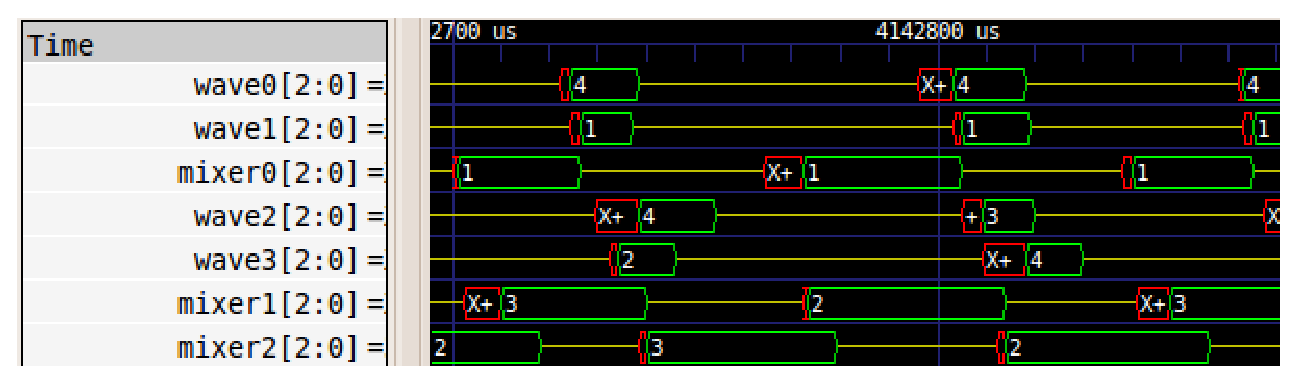
\includegraphics[width=\widefigure]{images/results_xeon/4KB_results_xeon_taskaff.eps}
\caption{\figurecaption{trace of benchmark execution on Xeon with buffer of 4KB using task-affinity}}
\label{fig:4KB_xeon_results_taskaff}
\end{figure}

\begin{figure}[htbp]
\centering
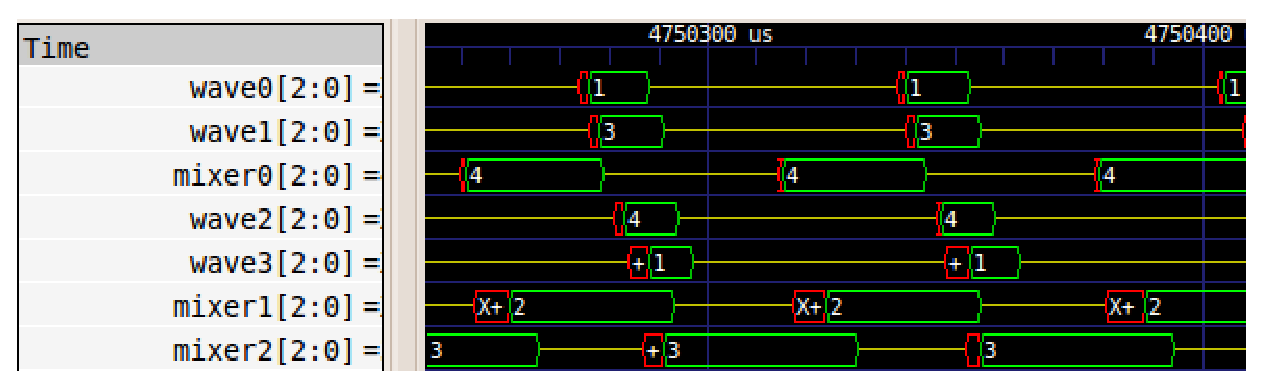
\includegraphics[width=\widefigure]{images/results_xeon/4KB_results_xeon_van.eps}
\caption{\figurecaption{trace of benchmark execution on Xeon with buffer of 4KB using vanilla}}
\label{fig:4KB_xeon_results_van}
\end{figure}

For what regard for speedups, in both Xeon and i7, the estimated average speedups overestimate the real parallelism performed by task-affinity, nevertheless
they are a good estimate. In fact, for Xeon, we have the estimated average speedup of $2.23$ and the real average speedup of $2.39$: they 
differ by $\sim 6\%$, Eq. \ref{eq:speedup_xeon_taskaff} and Tab. \ref{tab:final_time_speedup_xeon}. While for i7, we have an estimated average speedup of 
$2.45$ and a real average speedup of $2.50$: they differ by $\sim 2\%$, Eq. \ref{eq:speedup_i7_taskaff} and Tab. \ref{tab:final_time_speedup_i7}. Therefore, 
we can conclude that scheduling performed by task-affinity can be well approximated by the scheduling described in Fig. \ref{fig:ideal_scheduling}.

Instead, for vanilla, the estimated average speedups underestimate the real parallelism performed. In fact, for Xeon, we have an estimated average speedup 
of $1.86$ and a real average speedup of $2.19$: they differ by $\sim 18\%$, Eq. \ref{eq:speedup_xeon_van} and Tab. \ref{tab:final_time_speedup_xeon}. While 
for i7, we have an estimated average speedup of $2.11$ and a real average speedup of $2.26$: they differ by $\sim 7\%$, Eq. \ref{eq:speedup_i7_van} and 
Tab. \ref{tab:final_time_speedup_i7}. It is clear from these data, that parallelism of the scheduling performed by vanilla is greater with respect 
to parallelism of the ideal scheduling. In fact if we see Fig. \ref{fig:4KB_xeon_results_van} we note that there is a fraction of \textit{mixer2} that is 
executed concurrently with others \textit{waves}, while in ideal scheduling \textit{mixer2} should be executed alone.

\item[Migrations:] Number of migration is greatly increased with respect the vanilla. This is not due to architectural details or different buffer 
dimensions. This fact happens because, at each sample, \textit{waves}, \textit{mixer0} and \textit{mixer1} are excuted on the same CPUs. Since in the 
next sample \textit{waves} are woken up during the execution of \textit{mixer0} and \textit{mixer1}, they must be scheduled on CPUs different from which 
that have executed them in the previous sample. For this reason, at each sample, \textit{waves} are executed on different CPUs and, consequently, also 
other tasks are executed on different CPUs at each sample.

\item[Cache misses:] Because of worsening of L1 and LLC cache misses, Fig. \ref{fig:l1_load_store_xeon} and \ref{fig:l2_load_store_xeon}, on Intel Xeon 
predictability of the application is degradated, especially using small buffer dimension such as 4KB or 8KB, Fig. \ref{fig:time_avg_var_xeon}. LLC miss rate
is greatly increased in task-affinity, because, if a task migrates frequently between two different dies, at each migration it will have to warm up LLC 
cache and cache misses will occur. The same goes for L1 cache misses, also in that case a migration between CPUs that are in different dies increase L1 
miss rates. Nevertheless with dimension greater than 8KB and especially greater than 32KB predictability is improved, Fig. \ref{fig:time_avg_var_xeon}. On 
Intel i7, instead, thanks to the inclusive shared LLC, a core can access data contained in all caches of other cores, consequently, L1 and above all LLC 
cache misses are reduced, Fig \ref{fig:l1_load_store_i7} and \ref{fig:l2_load_store_i7}. The diminishing of cache misses impacts significantly on 
application predictability, Fig.\ref{fig:time_avg_var_i7}.

\item[Migration functions:] As we can see from Fig. \ref{fig:push_xeon} and \ref{fig:push_i7}, in both Xeon and i7, with task-affinity the number of calls 
to \texttt{push\_rt\_task} is greatly reduced with respect to vanilla. This fact happens because if a CPU is selected according to task-affinity criteria 
and the enqueued task with task-affinity is the next to be executed on the selected runqueue, \texttt{push\_rt\_task} for that runqueue is not called. 
Other tasks on that runqeueue that have to migrate will be moved by \texttt{pull\_rt\_task}. Instead, with \textit{pull\_rt\_task} task-affinity is not 
very effective, in fact, with task-affinity, \textit{pull\_rt\_task} executes more work than in vanilla, Fig. \ref{fig:pull_xeon} and \ref{fig:pull_i7}.

\begin{figure}[h]
  \lstset{basicstyle=\footnotesize, language=c, captionpos=b, frame=single,label=lis:steps}
  \lstinputlisting{pull_task.c}
  \label{code:pull_task_code}
  \caption{A portion of the \texttt{pull\_rt\_task} method}
\end{figure}

The explanation is simple: at line 1559, \texttt{pull\_rt\_task} checks for overloading runqueues. If in the system there 
is any overloaded runqueue, \textit{pull\_rt\_task} searches which runqueues are overloaded and tries to pull a task from them. With task-affinity, only 3 
\textit{waves} are executed concurrently and one \textit{wave} has to wait that \textit{mixer2} finishes. Therefore at each sample there is an overloaded 
runqueue in the system. For this reason, when \textit{pull\_rt\_task} is called, almost certainly it will enter in loop at line 1562 in order to pull tasks 
from an overloaded runqueue. With vanilla instead, all waves are executed concurrently, therefore there are less probabilities to have overloaded runqueues 
and thus \textit{pull\_rt\_task} will exit at line 1560. The overhead of \textit{pull\_rt\_task} influences predictability of an application especially with 
buffer of 4KB because execution time of each thread is relatively small.

\end{description}

%\begin{table}[tbp]
%\centering%
%\subfigure[ Value of A2S on Xeon ]{%
%\begin{tabular}{|l|c|c|c|}
%	\hline
%	& taskaff & vanilla & speedups \\ \hline
%	$4KB$ & 76,45 & 68,63 & -- \\ \hline
%	$8KB$ & 100,43 & 104,55 & 4\%\\ \hline
%	$16KB$ & 160,15 & 178,27 & 10\%\\ \hline
%	$32KB$  & 276,84 & 319,85 & 13\%\\ \hline
%	$64KB$  & 519,35 & 610,35 & 15\%\\ \hline
%\end{tabular}
%\label{tab:speedup_xeon}
%}
%\subfigure[ Values of A2S on i7 ]{%
%\begin{tabular}{|l|c|c|c|}
%	\hline
%	& taskaff & vanilla & speedups \\ \hline
%	$4KB$ & 70,47 & 79,91 & 12\%\\ \hline
%	$8KB$ & 118,32 & 148,34 & 20\%\\ \hline
%	$16KB$ & 223,61 & 284,8 & 21\%\\ \hline
%	$32KB$  & 437,76 & 548,08 & 20\%\\ \hline
%	$64KB$  & 868,97 & 987,7 & 12\%\\ \hline
%\end{tabular}
%\label{tab:speedup_i7}
%}
%\label{tab:final_speedup}
%\caption{Comparison between task-affinity and vanilla on Intel Xeon and Intel i7}
%\end{table}

In conclusion, to get a sense of how task-affinity improves the performance of the benchmark, look at table \ref{tab:final_time_speedup_xeon}, where are reported 
values of metric A2S (Eq. \ref{eq:metric_rt}) used to characterize how task-affinity improve throughput and predictability with respect to vanilla. As we 
can see, task-affinity is well exploited by Intel i7, look at \ref{tab:final_time_i7}, while on Intel Xeon we have some advantage with buffer greater than 4KB. Speedups are calculated using
Eq. \ref{eq:miss_rate} 

%%%%%%%%%%%%%%%%%%%%%%%%%%%%%%%%%%%%%%%%%%%%%%%%%%%%%%%%%%%%%%%%%%%%%%%%%%%%%
\section{Intel Xeon}

\begin{figure}[htbp]
\centering
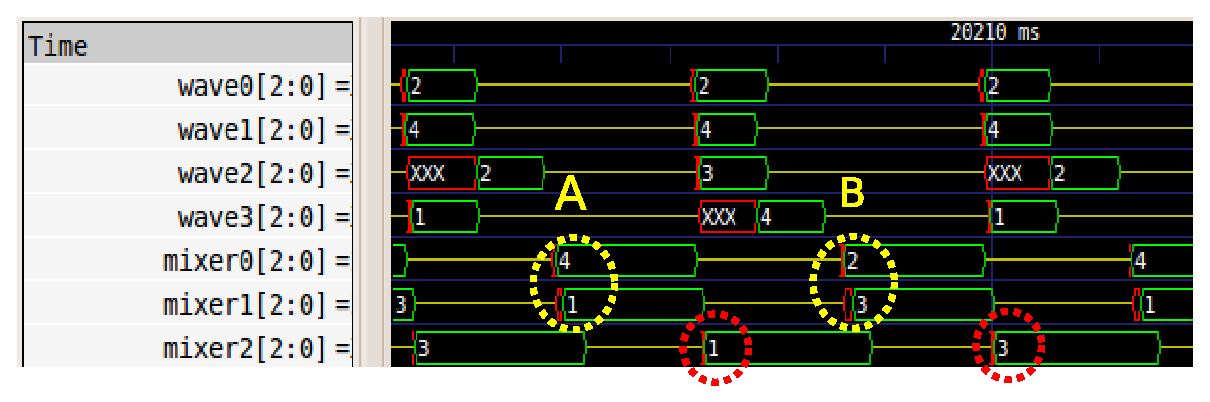
\includegraphics[width=\widefigure]{images/results_xeon/final_xeon.eps}
\caption{\figurecaption{Scheduling performed by task-affinity on Intel Xeon.}}
\label{fig:final_xeon}
\end{figure}

As we can see in Fig. \ref{fig:final_xeon}, the scheduling performed is correct. We see that \textit{mixer2} can precede one of the waves and improve 
parallelism. We see that \textit{mixer0} chooses the best cpu in term of temporal locality, for example: in step A \textit{mixer0} chooses CPU4 and not 
CPU2, because on CPU2 was executed \textit{wave2}, therefore L1 cache could be dirty, instead on CPU4 the last task executed is \textit{wave1}, therefore 
L1 cache should be clean. Also in step B, it is possible to note how \textit{mixer0} take care about the last task executed on CPU4 choosing CPU2.

\begin{table}[tbp]
\centering%
\subfigure[ Average of execution times of each task on serialized execution (us). The speedups for parallel execution are computed as: serialized execution 
time divided by sample time. ]%
{
%\begin{tabular}{|p{1.0cm}|p{1.4cm}|p{1.4cm}|p{1.4cm}|p{2cm}|}
\begin{tabular}{|l|r|r|r|r|r|r|r|r|}
	\hline
	& $waves$ & $mixer_{0,1}$ & $mixer_{2}$ & serialized & \multicolumn{2}{|c|}{Sample time} & \multicolumn{2}{|c|}{Speedup} \\ 
	       &        &        &        & exec. time &  va    &   ta    &  va  & ta   \\ \hline	
	 $4KB$ & 12.18  & 29.59  & 38.84  & 146.76  & 61.58  &  63.08  & 2.38 & 2.33 \\ \hline
	 $8KB$ & 17.74  & 42.72  & 55.57  & 211.98  & 95.54  &  90.60  & 2.22 & 2.34 \\ \hline
	$16KB$ & 31.47  & 70.35  & 88.53  & 355.13  & 165.23 &  150.00 & 2.15 & 2.37 \\ \hline
	$32KB$ & 60.12  & 128.72 & 155.34 & 653.27  & 306.69 &  266.42 & 2.13 & 2.45 \\ \hline
	$64KB$ & 115.42 & 246.2  & 285.62 & 1239.69 & 592.30 &  502.09 & 2.09 & 2.47 \\ \hline
     $Average$ &        & 	 & 	  & 	    & 	     &	       & 2.39 & 2.19 \\ \hline
\end{tabular}
\label{tab:task_time_xeon}
}

\subfigure[Portions of serialized execution]%
{
\begin{tabular}{|l|r|r|r|r|r|r|r|r|}
	\hline	
	& \multicolumn{2}{|c|}{$P_{1}$} & \multicolumn{2}{|c|}{$P_{2}$} & \multicolumn{2}{|c|}{$P_{3}$} & \multicolumn{2}{|c|}{$P_{4}$} \\
  	       & va   & ta   & va   & ta   & va   & ta   & va & ta   \\ \hline
	 $4KB$ & 40\% & 40\% & 33\% & 33\% & 26\% & 16\% & -- & 10\% \\ \hline
	 $8KB$ & 39\% & 40\% & 33\% & 33\% & 26\% & 16\% & -- &  9\% \\ \hline
	$16KB$ & 40\% & 40\% & 35\% & 36\% & 25\% & 18\% & -- &  7\% \\ \hline
	$32KB$ & 40\% & 39\% & 37\% & 37\% & 24\% & 18\% & -- &  5\% \\ \hline
	$64KB$ & 40\% & 40\% & 37\% & 37\% & 23\% & 18\% & -- &  4\% \\ \hline
     $Average$ & 40\% & 40\% & 35\% & 35\% & 25\% & 18\% & -- &  7\% \\ \hline
\end{tabular}
\label{tab:portion_van_xeon}
}

\subfigure[ Sample production time (us) ]%
{
\begin{tabular}{|l|r|r|r|r|r|r|r|}
	\hline
	& \multicolumn{3}{|c|}{taskaff} & \multicolumn{3}{|c|}{vanilla} & A2S\\
	      & avg    & var   & A2S    & avg    & var   & A2S    & Speedup \\ \hline
	$4KB$ & 63.08  & 44.7  & 76.45  & 61.58  & 12.42 & 68.63  & -11\%\\ \hline
	$8KB$ & 90.6   & 24.18 & 100.43 & 95.54  & 20.31 & 104.55 & 4\%\\ \hline
       $16KB$ & 150.00 & 25.75 & 160.15 & 165.23 & 42.47 & 178.27 & 10\%\\ \hline
       $32KB$ & 266.42 & 27.17 & 276.84 & 306.69 & 43.31 & 319.85 & 13\%\\ \hline
       $64KB$ & 502.09 & 74.54 & 519.35 & 592.3  & 81.45 & 610.35 & 15\%\\ \hline
\end{tabular}
\label{tab:final_time_xeon}
}

\label{tab:final_time_speedup_xeon}
\caption{Data used to calculate speedups of task-affinity and vanilla on Xeon}
\end{table}

According the showed data, Tab. \ref{tab:final_time_speedup_xeon}, it possible to estimate the average speedups for task-affinity and vanilla.

\begin{equation}
  Speedup_{taskaff} = \left( \frac{0.4}{2} + \frac{0.35}{4} + \frac{0.18}{2} + \frac{0.07}{1}\right)^{-1} = 2.23
\label{eq:speedup_xeon_taskaff}
\end{equation}

\begin{equation}
  Speedup_{vanilla} = \left(\frac{0.4}{2} + \frac{0.35}{4} + \frac{0.25}{1} \right)^{-1} = 1.86
\label{eq:speedup_xeon_van}
\end{equation}

\begin{figure}[htbp]
\centering
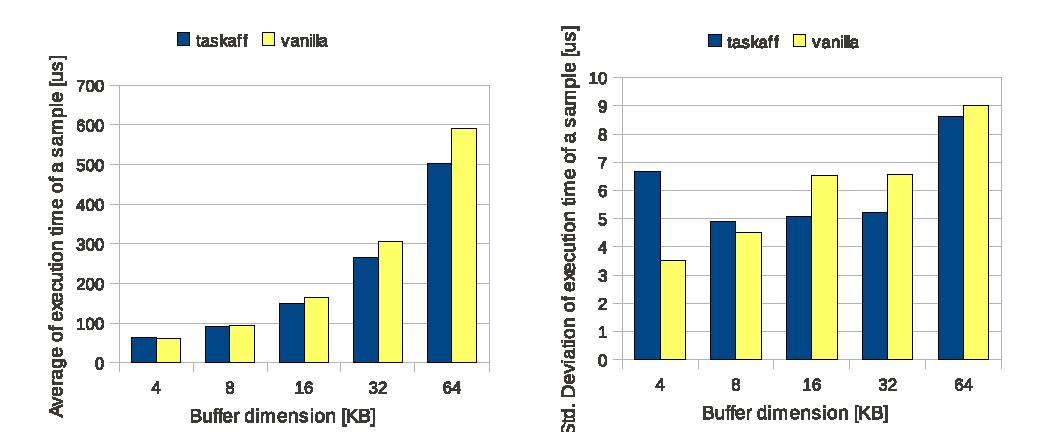
\includegraphics[width=\widefigure]{images/results_xeon/time_avg_var_Xeon.eps}
\caption{\figurecaption{Average and Variance of execution time of a sample on Xeon}}
\label{fig:time_avg_var_xeon}
\end{figure}

\begin{figure}[htbp]
\centering
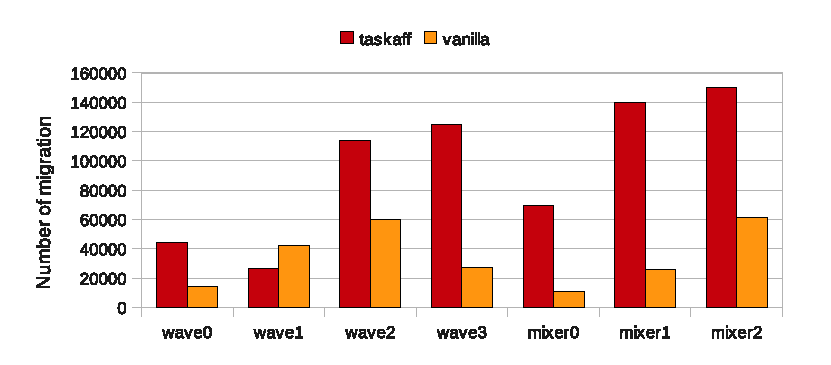
\includegraphics[width=\widefigure]{images/results_xeon/migration_xeon.eps}
\caption{\figurecaption{task migration on Xeon}}
\label{fig:migration_xeon}
\end{figure}

\begin{figure}[htbp]
\centering
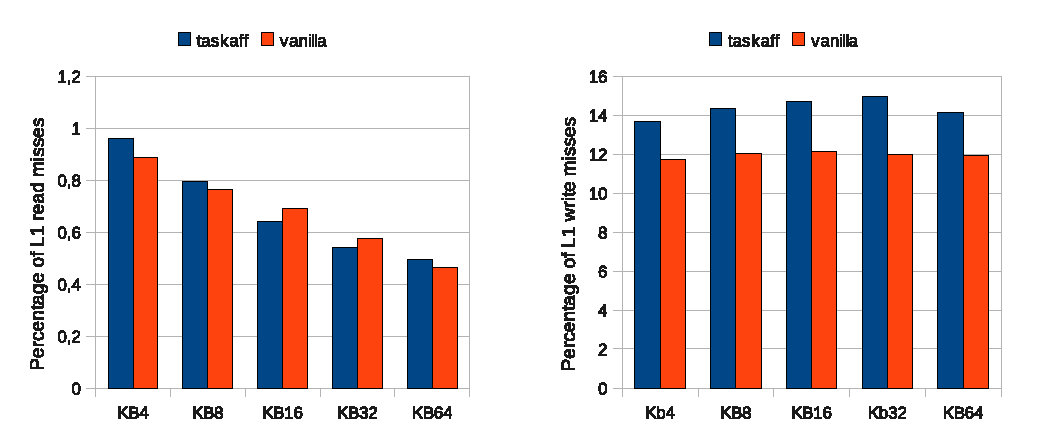
\includegraphics[width=\widefigure]{images/results_xeon/l1_load_store_xeon.eps}
\caption{\figurecaption{L1 Read and Write misses on Xeon}}
\label{fig:l1_load_store_xeon}
\end{figure}

\begin{figure}[htbp]
\centering
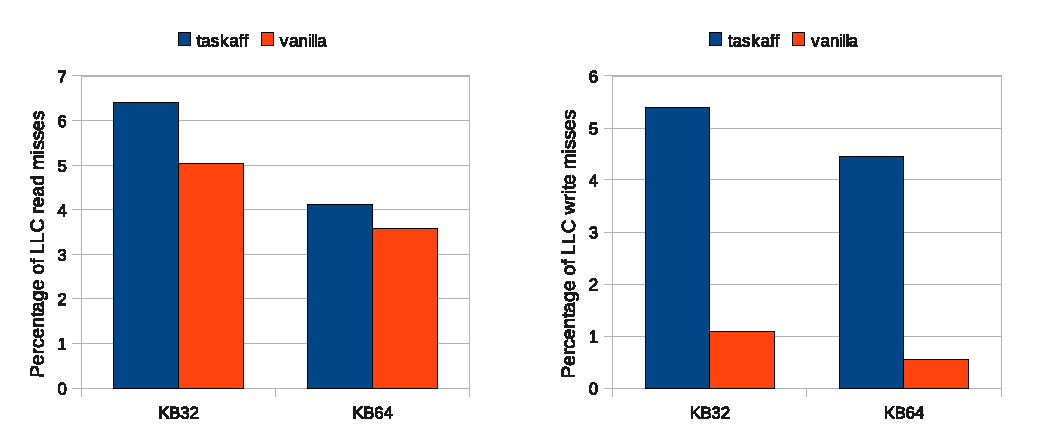
\includegraphics[width=\widefigure]{images/results_xeon/l2_load_store_xeon.eps}
\caption{\figurecaption{LLC Read and Write misses on Xeon}}
\label{fig:l2_load_store_xeon}
\end{figure}

\begin{figure}[htbp]
\centering
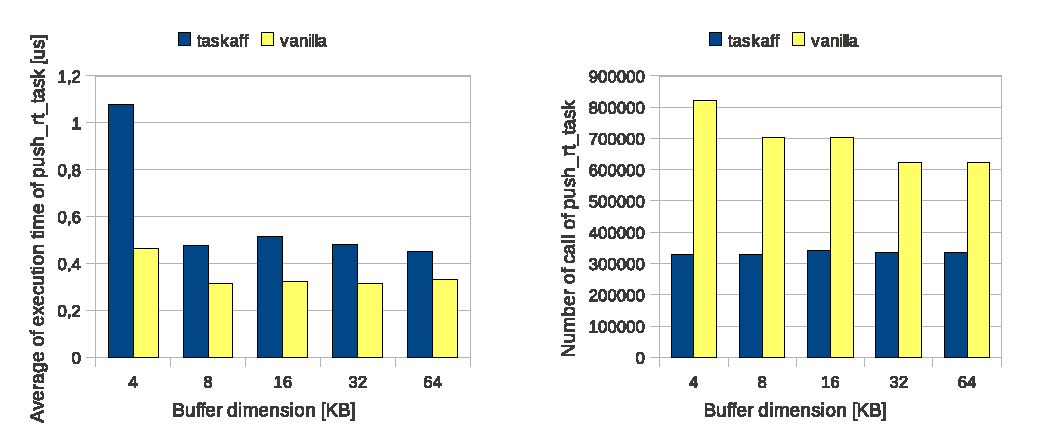
\includegraphics[width=\widefigure]{images/results_xeon/push_xeon.eps}
\caption{\figurecaption{Average of execution time of a call to push\_rt\_task and number of call to push\_rt\_task on Xeon}}
\label{fig:push_xeon}
\end{figure}

\begin{figure}[htbp]
\centering
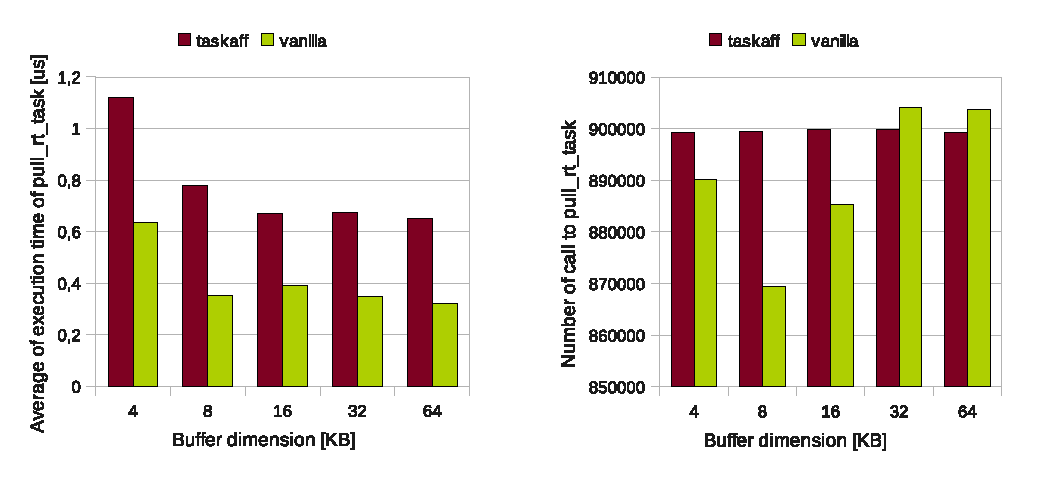
\includegraphics[width=\widefigure]{images/results_xeon/pull_xeon.eps}
\caption{\figurecaption{Average of execution time of a call to pull\_rt\_task and number of call to pull\_rt\_task on Xeon}}
\label{fig:pull_xeon}
\end{figure}

\newpage
%%%%%%%%%%%%%%%%%%%%%%%%%%%%%%%%%%%%%%%%%%%%%%%%%%%%%%%%%%%%%%%%%%%%%%%%%%%%%
\section{Intel i7}

\begin{figure}[htbp]
\centering
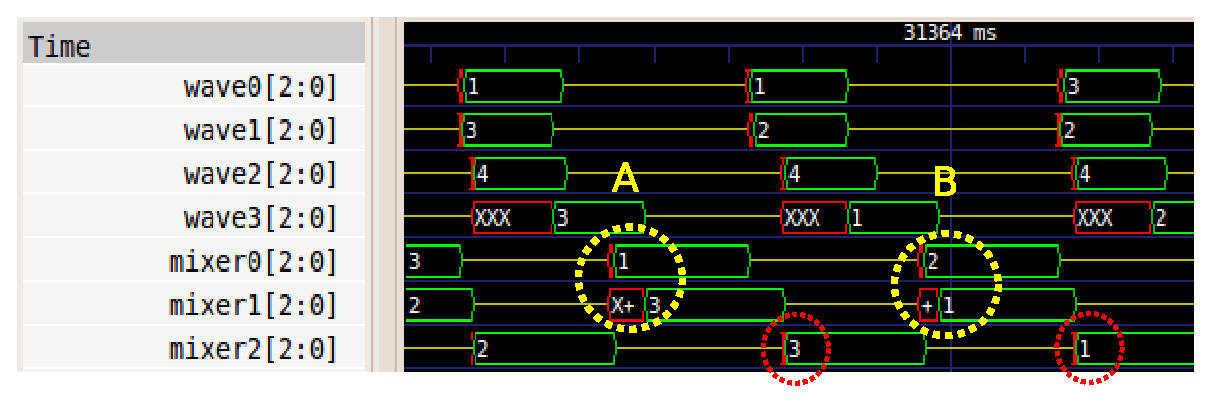
\includegraphics[width=\widefigure]{images/results_i7/final_i7.eps}
\caption{\figurecaption{Scheduling performed by task-affinity.}}
\label{fig:trace_i7}
\end{figure}

We can see from Fig.\ref{fig:trace_i7}, that also in this case the scheduling performed can be approximated with the ideal scheduling, Fig.
\ref{fig:ideal_scheduling}. We can see how in step A and B \textit{mixers} choose the correct CPUs according to their task-affinity relationships.

Also in this case, according to recorded measurement the estimated average speedups are:

\begin{equation}
  Speedup_{taskaff} = \left(\frac{0.32}{2} + \frac{0.49}{4} + \frac{0.13}{2} + \frac{0.06}{1} \right)^{-1} = 2.45
\label{eq:speedup_i7_taskaff}
\end{equation}

\begin{equation}
  Speedup_{vanilla} = \left(\frac{0.32}{2} + \frac{0.49}{4} + \frac{0.19}{1} \right)^{-1} = 2.11
\label{eq:speedup_i7_van}
\end{equation}

\begin{table}[tbp]
\centering%
\subfigure[ Average of execution times of each task on serialized execution (us). The speedups for parallel execution are computed as: serialized execution 
time divided by sample time. ]%
{
%\begin{tabular}{|p{1.0cm}|p{1.4cm}|p{1.4cm}|p{1.4cm}|p{2cm}|}
\begin{tabular}{|l|r|r|r|r|r|r|r|r|}
	\hline
	& $waves$ & $mixer_{0,1}$ & $mixer_{2}$ & serialized & \multicolumn{2}{|c|}{Sample time} & \multicolumn{2}{|c|}{Speedup} \\ 
	       &        &        &        & exec. time &  va    &   ta   &  va   & ta   \\ \hline	
	 $4KB$ & 17.86  & 27.31  & 29.25  & 155.31     & 68.25  & 61.44  &  2.28 & 2.53 \\ \hline
	 $8KB$ & 33.17  & 46.39  & 51.88  & 277.32     & 122.42 & 108.22 &  2.27 & 2.56 \\ \hline
	$16KB$ & 63.65  & 82.49  & 96.54  & 516.11     & 236.35 & 206.03 &  2.18 & 2.51 \\ \hline
	$32KB$ & 124.85 & 156.46 & 182.30 & 994.59     & 444.38 & 401.53 &  2.24 & 2.48 \\ \hline
	$64KB$ & 250.27 & 279.39 & 356.96 & 1916.82    & 826.83 & 793.50 &  2.32 & 2.42 \\ \hline
     $Average$ &        & 	 & 	  & 	       & 	&        &  2.26 & 2.50 \\ \hline
\end{tabular}
\label{tab:task_time_i7}
}

\subfigure[Portions of serialized execution]%
{
\begin{tabular}{|l|r|r|r|r|r|r|r|r|}
	\hline	
	& \multicolumn{2}{|c|}{$P_{1}$} & \multicolumn{2}{|c|}{$P_{2}$} & \multicolumn{2}{|c|}{$P_{3}$} & \multicolumn{2}{|c|}{$P_{4}$} \\
  	       & va   & ta   & va   & ta   & va   & ta   & va & ta   \\ \hline
	 $4KB$ & 35\% & 35\% & 47\% & 47\% & 18\% & 14\% & -- & 7\% \\ \hline
	 $8KB$ & 33\% & 33\% & 48\% & 48\% & 19\% & 14\% & -- & 7\% \\ \hline
	$16KB$ & 32\% & 32\% & 49\% & 49\% & 18\% & 12\% & -- & 6\% \\ \hline
	$32KB$ & 31\% & 31\% & 51\% & 51\% & 19\% & 12\% & -- & 5\% \\ \hline
	$64KB$ & 29\% & 29\% & 52\% & 52\% & 19\% & 12\% & -- & 4\% \\ \hline
     $Average$ & 32\% & 32\% & 49\% & 49\% & 19\% & 13\% & -- & 6\% \\ \hline
\end{tabular}
\label{tab:portion_van_i7}
}

\subfigure[ Sample production time (us) ]%
{
\begin{tabular}{|l|r|r|r|r|r|r|r|}
	\hline
	& \multicolumn{3}{|c|}{taskaff} & \multicolumn{3}{|c|}{vanilla} & A2S\\
	      & avg    & var     & A2S    & avg    & var     & A2S    & Speedup \\ \hline
	$4KB$ & 61.44  & 20.38   & 70.47  & 68.25  & 34.02   & 79.91  & 12\%    \\ \hline
	$8KB$ & 108.22 & 25.54   & 118.32 & 122.42 & 167.94  & 148.34 & 20\%    \\ \hline
       $16KB$ & 206.03 & 77.33   & 223.61 & 236.35 & 586.69  & 284.80 & 21\%    \\ \hline
       $32KB$ & 401.53 & 328.09  & 437.76 & 444.38 & 2688.34 & 548.08 & 20\%    \\ \hline
       $64KB$ & 793.50 & 1423.98 & 868.97 & 826.83 & 6469.23 & 987.70 & 12\%    \\ \hline
\end{tabular}
\label{tab:final_time_i7}
}
\label{tab:final_time_speedup_i7}
\caption{Data used to calculate speedups of task-affinity and vanilla on i7}
\end{table}

\begin{figure}[htbp]
\centering
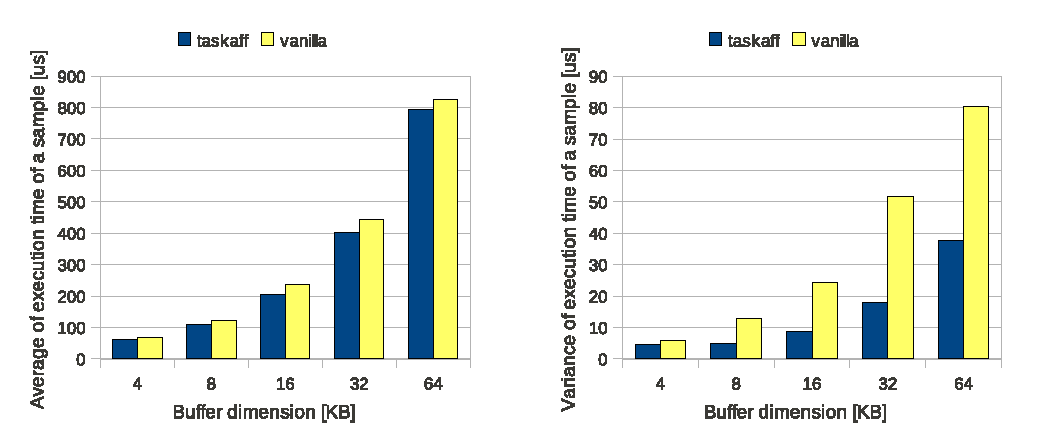
\includegraphics[width=\widefigure]{images/results_i7/time_avg_var_i7.eps}
\caption{\figurecaption{Average and Variance of execution time of a sample on i7}}
\label{fig:time_avg_var_i7}
\end{figure}

\begin{figure}[htbp]
\centering
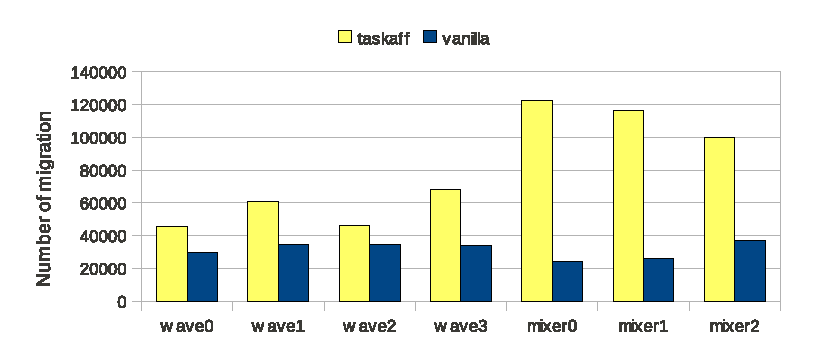
\includegraphics[width=\widefigure]{images/results_i7/migration_i7.eps}
\caption{\figurecaption{task migration on i7}}
\label{fig:migration_i7}
\end{figure}

\begin{figure}[htbp]
\centering
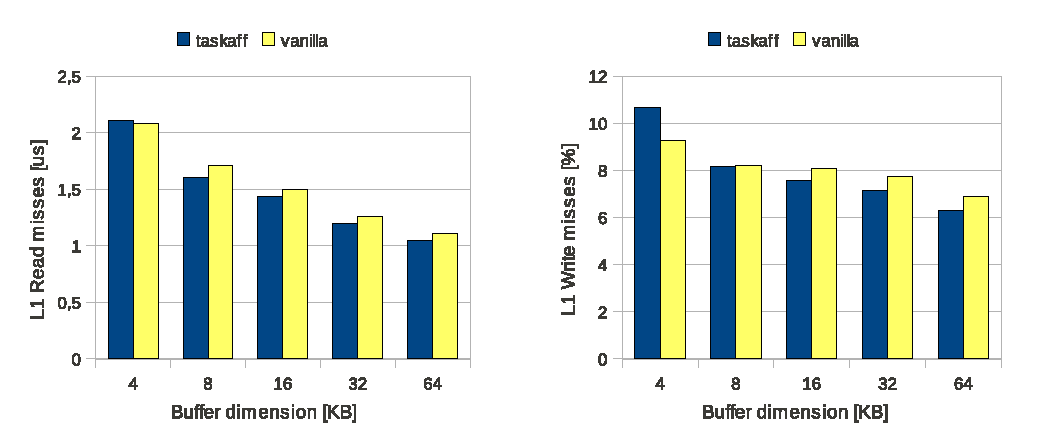
\includegraphics[width=\widefigure]{images/results_i7/l1_load_store_i7.eps}
\caption{\figurecaption{L1 Read and Write misses on i7}}
\label{fig:l1_load_store_i7}
\end{figure}

\begin{figure}[htbp]
\centering
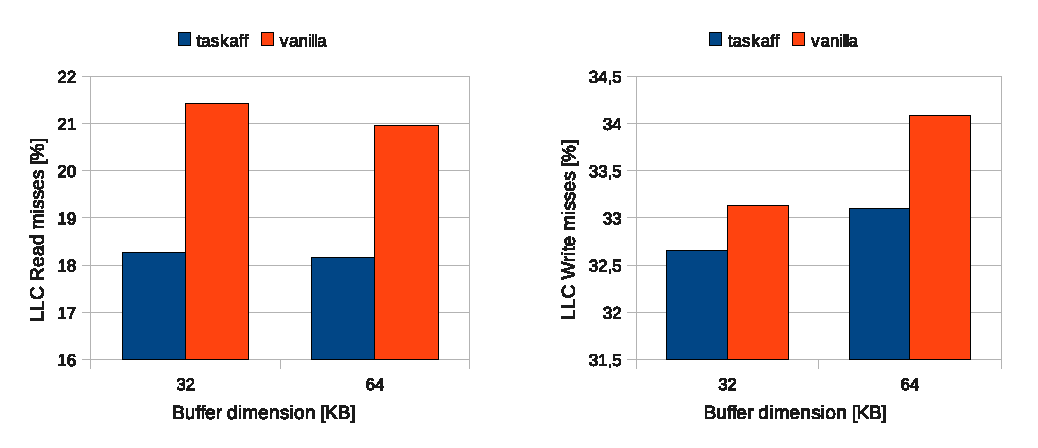
\includegraphics[width=\widefigure]{images/results_i7/l3_load_store_i7.eps}
\caption{\figurecaption{LLC Read and Write misses on i7}}
\label{fig:l2_load_store_i7}
\end{figure}

\begin{figure}[htbp]
\centering
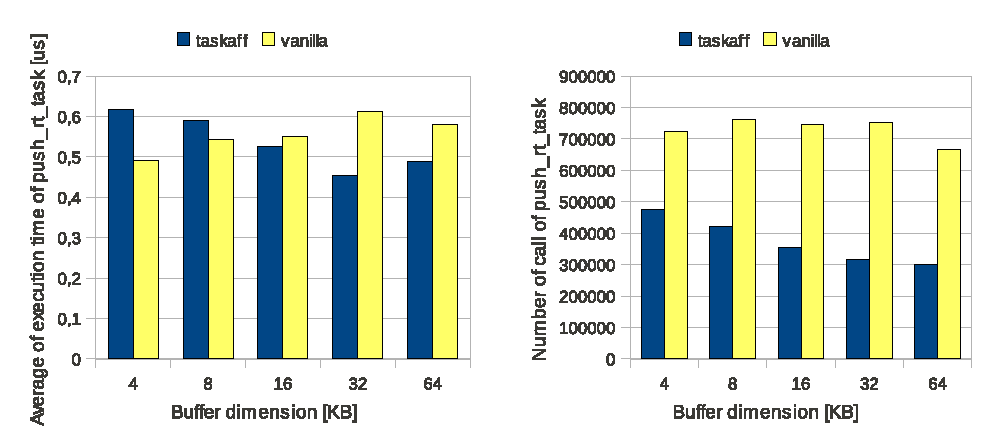
\includegraphics[width=\widefigure]{images/results_i7/push_i7.eps}
\caption{\figurecaption{Average of execution time of a call to push\_rt\_task and number of call to push\_rt\_task on i7}}
\label{fig:push_i7}
\end{figure}

\begin{figure}[htbp]
\centering
\includegraphics[width=\widefigure]{images/results_i7/pull_i7.eps}
\caption{\figurecaption{Average of execution time of a call to pull\_rt\_task and number of call to pull\_rt\_task on i7}}
\label{fig:pull_i7}
\end{figure}

